\section{Heart and Pacemaker Basics}
\label{basics}
In this section, we review basic concepts related to the heart and its electrical conduction system which interacts with the pacemaker. 
In-depth material of cardiac electro-physiology can be found in \cite{fogoros}. 

\subsection{Basics of Cardiac Electrophysiology Operation}
The coordinated contraction of the heart is governed by its Electrical Conduction System (see \ref{conduction}). The Sinoatrial (SA) node, which is a collection of specialized tissue at the upper right atrium, spontaneously generates periodical electrical pulses that can cause muscle contraction. 
The SA node acts as the natural pacemaker of the heart. 
The electrical pulses first cause both atria to contract, forcing the blood into the ventricles. 
The electrical conduction is then delayed at the Atrioventricular (AV) node, allowing the ventricles to fill fully. Finally, the fast-conducting His-Pukinje system spreads the electrical activation within both ventricles, causing simultaneous contraction of the ventricular muscles, and pumps the blood out of the heart. 
Appropriate timing is key to proper heart rhythm.

\begin{figure}
  	\begin{center}
    	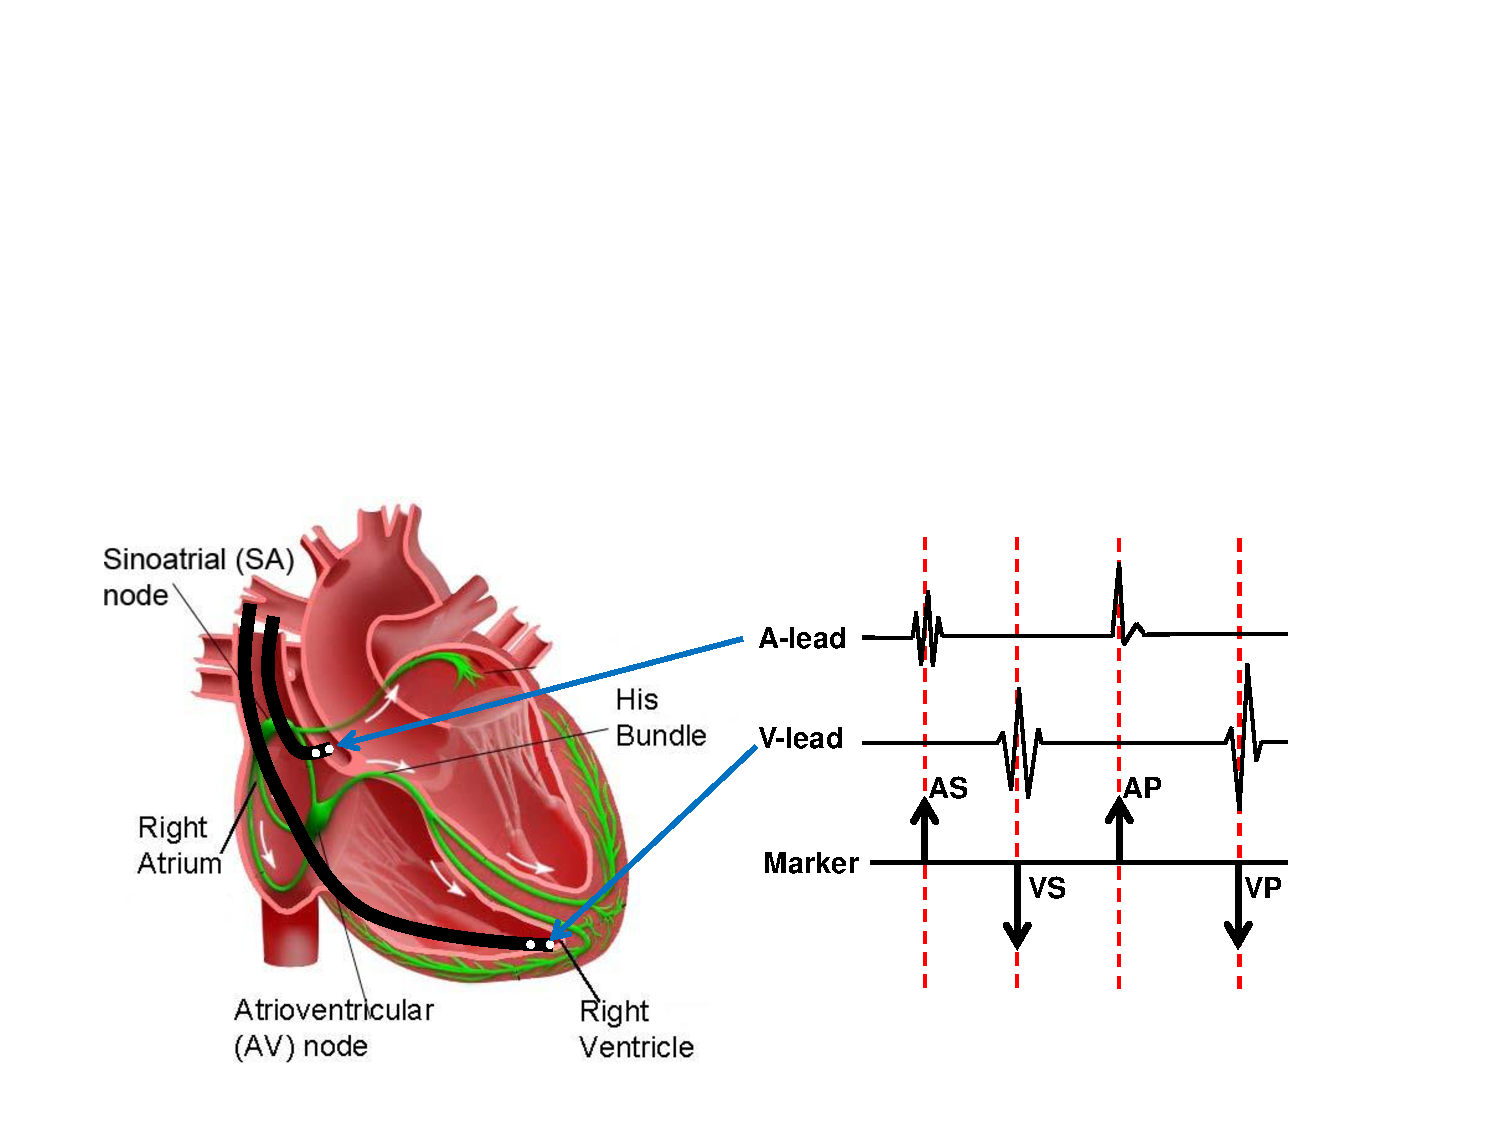
\includegraphics[width=0.45\textwidth]{figures/egm.pdf}
  	\end{center}
	\caption{\small (a) Electrical Conduction System of the Heart and pacemaker leads location. (b) Electrical signal sensed from the pacemaker leads are converted to event markers (AS,VS). Pacemaker delivers electrical pacing (AP,VP) from corresponding leads when heart rate is slow.}
	\label{fig:conduction}
\end{figure}

Due to various factors such as aging and disease, the conduction properties of heart tissue may change. 
These changes often cause timing anomalies in heart rhythm, thus decreasing the blood pumping efficiency of the heart. These timing anomalies are referred to as \emph{arrhythmias}.  

%\subsection{Interfacing the Heart with the Pacemaker}
\label{interfacingHeartPM}


